\documentclass[11pt]{article}
\usepackage[a4paper,margin=1in]{geometry}
\usepackage[T1]{fontenc}
\usepackage[utf8]{inputenc}
\usepackage{lmodern,microtype,booktabs,tabularx,multirow,array,xcolor,amsmath,amssymb,graphicx,caption,float,enumitem,tikz}
\usetikzlibrary{arrows.meta,positioning,fit,calc,backgrounds}
\definecolor{navy}{HTML}{102A43}
\definecolor{blue}{HTML}{2F80ED}
\definecolor{teal}{HTML}{00A6A6}
\definecolor{orange}{HTML}{F2994A}
\definecolor{lightblue}{HTML}{EEF5FF}
\definecolor{lightteal}{HTML}{E8F8F5}
\newcommand{\poc}{\textsc{POC}}
\title{Context-Aware MTN for Pedestrian Trajectory Prediction\\\large A CPU-based Proof-of-Concept on IDD-PeD}
\author{Author names to be added}
\date{Draft -- \today}
\begin{document}
\maketitle
\begin{abstract}
This draft documents a context-aware extension of MTN for pedestrian trajectory prediction on IDD-PeD. The proposed proof-of-concept architecture, C4 Context-Aware MTN, augments observed pedestrian trajectories with six native context sources and shares only encoder self-attention projections across depth. The draft reports a matched CPU Farneback evaluation and explicitly distinguishes it from the authors' RAFT-based benchmark. Dynamic Multimodal Fusion is included as a separate evaluated candidate rather than part of the proposed C4 architecture.
\end{abstract}
\section{Proposed Methodology}
\label{sec:method}

\subsection{Problem formulation and MTN backbone}
Given an observed pedestrian bounding-box trajectory $\mathbf{X}_{obs}\in\mathbb{R}^{B\times15\times4}$, the objective is to predict future bounding boxes $\widehat{\mathbf{X}}_{fut}\in\mathbb{R}^{B\times45\times4}$. The MTN backbone embeds the observed trajectory and adds positional encoding, producing a sequence of width $32$, i.e., $[B,15,32]$. Three MTN encoder layers generate trajectory memory $\mathbf{M}\in\mathbb{R}^{B\times15\times32}$. The original flow-related decoder paths are retained; the decoder output is mapped to four bounding-box coordinates and combined with the final observed-box residual. The dataset protocol and baseline implementation materials follow the official IDD-PeD release \cite{iddped2025,iddped_repo}.

\subsection{Native IDD-PeD context branch}
\label{sec:context}
The first contribution is a context branch built only from six verified native IDD-PeD sources: \emph{intersection\_type}, \emph{signalized\_type}, \emph{road\_type}, \emph{location\_type}, \emph{motion\_direction}, and observed \emph{occlusion}. Day/night and illumination are not included because they were not verified as inputs of the implemented final context branch.

Each source is represented by a 16-dimensional embedding. The five static labels use independent embedding lookups; the observed occlusion history is embedded and mean-pooled over observed steps. The six vectors are concatenated to a 96-dimensional context feature, then projected to the MTN width of 32. The original context-admission gate receives the context representation together with the final observed bounding box, and yields a gated context token $\mathbf{c}\in\mathbb{R}^{B\times1\times32}$. The token is appended \emph{after} the trajectory encoder, yielding augmented decoder memory $[B,16,32]$. This preserves the baseline trajectory memory while allowing the decoder's existing source-attention path to condition on scene context.

\subsection{C4: cross-layer encoder self-attention weight sharing}
\label{sec:c4}
The second contribution is selective cross-layer sharing in the trajectory encoder. C4 aliases only the Q/K/V/O projections of \texttt{EncoderLayer.self\_attn} across encoder layers 0--2. The encoder's \texttt{src\_attn}, \texttt{cross\_attn}, feed-forward networks, normalisation layers, decoder modules, context branch, and output head remain independent. Therefore, C4 is not full layer sharing.

This choice reduces the number of unique parameters while preserving the three sequential encoder-layer executions. It must consequently be interpreted as a parameter-footprint technique, not as a FLOP-reduction claim. The measured CPU latency is reported separately in Section~\ref{sec:results}.

\begin{figure*}[t]
\centering
\resizebox{\textwidth}{!}{% Colourful paper-style overview. Text is intentionally short; detail belongs in the caption.
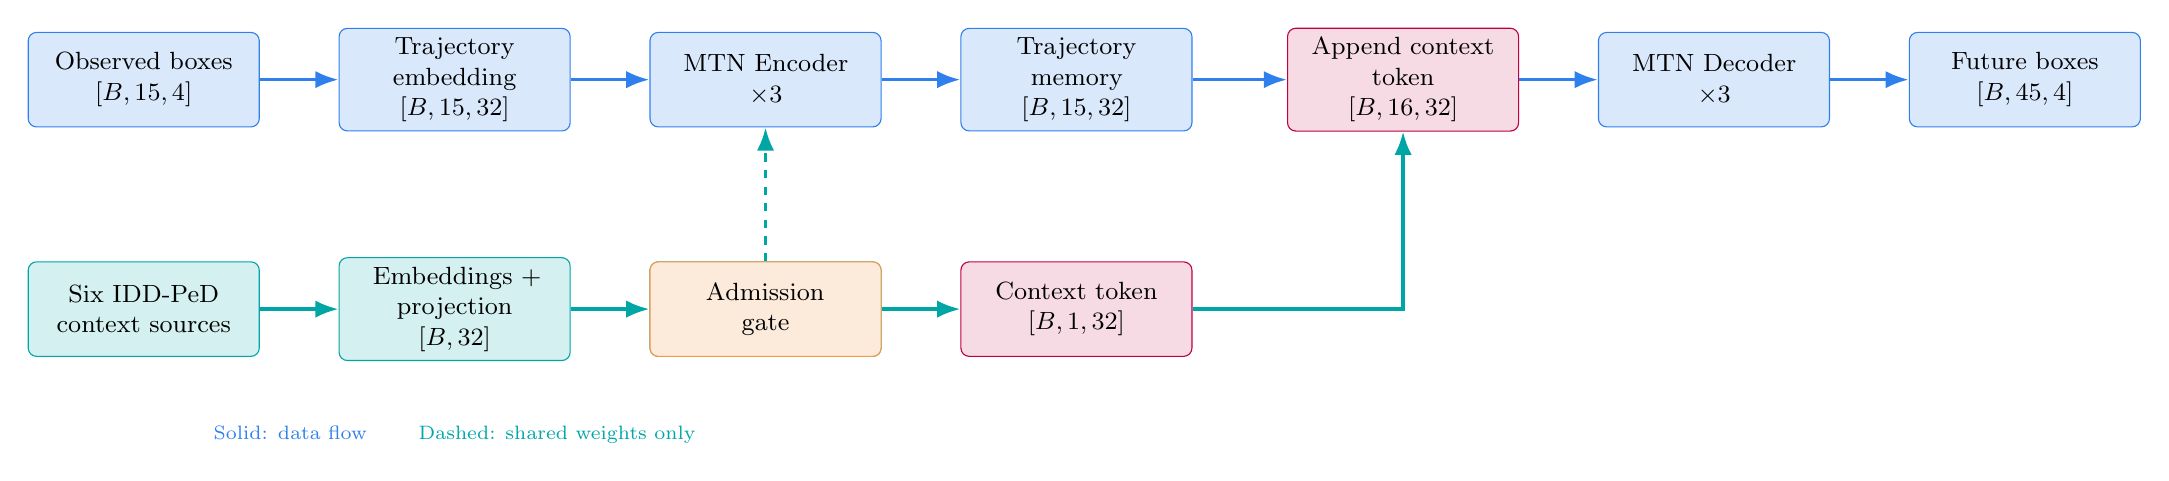
\begin{tikzpicture}[font=\small,
 t/.style={draw=blue,fill=blue!18,rounded corners=3pt,minimum height=12mm,text width=27mm,align=center},
 c/.style={draw=teal,fill=teal!17,rounded corners=3pt,minimum height=12mm,text width=27mm,align=center},
 g/.style={draw=orange,fill=orange!20,rounded corners=3pt,minimum height=12mm,text width=27mm,align=center},
 o/.style={draw=purple,fill=purple!14,rounded corners=3pt,minimum height=12mm,text width=27mm,align=center},
 a/.style={-Latex,very thick,draw=blue},ca/.style={-Latex,very thick,draw=teal},da/.style={-Latex,dashed,very thick,draw=teal}]
\node[t] (x) {Observed boxes\\$[B,15,4]$};
\node[t,right=10mm of x] (e) {Trajectory\\embedding\\$[B,15,32]$};
\node[t,right=10mm of e] (enc) {MTN Encoder\\$\times 3$};
\node[t,right=10mm of enc] (m) {Trajectory memory\\$[B,15,32]$};
\node[o,right=12mm of m] (aug) {Append context\\token\\$[B,16,32]$};
\node[t,right=10mm of aug] (dec) {MTN Decoder\\$\times3$};
\node[t,right=10mm of dec] (y) {Future boxes\\$[B,45,4]$};
\draw[a] (x)--(e);\draw[a](e)--(enc);\draw[a](enc)--(m);\draw[a](m)--(aug);\draw[a](aug)--(dec);\draw[a](dec)--(y);
\node[c,below=17mm of enc] (share) {C4 shared\\Q / K / V / O};
\draw[da](share)--(enc);
\node[c,below=17mm of x] (scene) {Six IDD-PeD\\context sources};
\node[c,right=10mm of scene] (ctx) {Embeddings +\\projection\\$[B,32]$};
\node[g,right=10mm of ctx] (gate) {Admission\\gate};
\node[o,right=10mm of gate] (token) {Context token\\$[B,1,32]$};
\draw[ca](scene)--(ctx);\draw[ca](ctx)--(gate);\draw[ca](gate)--(token);\draw[ca](token.east)-| (aug.south);
\node[font=\scriptsize,text=blue,below=7mm of ctx] {\textcolor{blue}{Solid: data flow} \qquad \textcolor{teal}{Dashed: shared weights only}};
\end{tikzpicture}
}
\caption{Colour-coded overview of the proposed C4 Context-Aware MTN. Blue: trajectory pathway; teal: native context pathway; orange: admission decision; purple: memory augmentation. Dashed teal denotes shared weights only.}
\label{fig:c4-overview}
\end{figure*}

\begin{figure*}[t]
\centering
\resizebox{\textwidth}{!}{% Context branch as a compact, colourful conceptual mechanism.
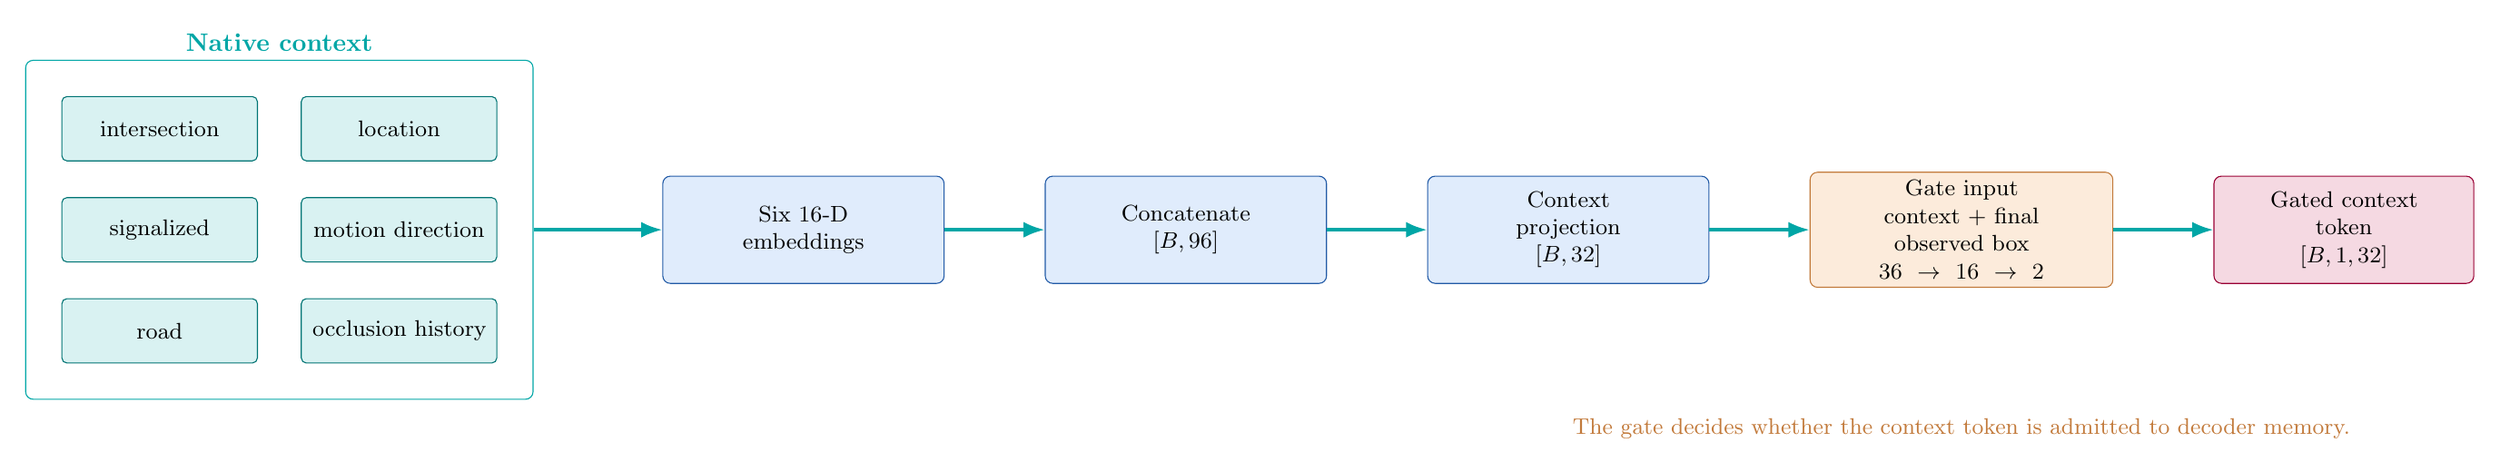
\begin{tikzpicture}[font=\small,
 s/.style={draw=teal!70!black,fill=teal!15,rounded corners=2pt,minimum height=9mm,text width=25mm,align=center},
 p/.style={draw=blue!70!black,fill=blue!15,rounded corners=3pt,minimum height=15mm,text width=37mm,align=center},
 g/.style={draw=orange!80!black,fill=orange!20,rounded corners=3pt,minimum height=15mm,text width=40mm,align=center},
 tok/.style={draw=purple!80!black,fill=purple!15,rounded corners=3pt,minimum height=15mm,text width=34mm,align=center},
 a/.style={-Latex,very thick,draw=teal}]
\node[s] (a1) {intersection};\node[s,below=5mm of a1](a2){signalized};\node[s,below=5mm of a2](a3){road};
\node[s,right=6mm of a1](a4){location};\node[s,below=5mm of a4](a5){motion direction};\node[s,below=5mm of a5](a6){occlusion history};
\node[draw=teal,rounded corners=3pt,inner sep=5mm,fit=(a1)(a6),label={[font=\bfseries,text=teal]above:Native context}] (src) {};
\node[p,right=18mm of src] (emb) {Six 16-D\\embeddings};
\node[p,right=14mm of emb] (cat) {Concatenate\\$[B,96]$};
\node[p,right=14mm of cat] (proj) {Context\\projection\\$[B,32]$};
\node[g,right=14mm of proj] (gate) {Gate input\\context + final\\observed box\\$36\rightarrow16\rightarrow2$};
\node[tok,right=14mm of gate] (tok) {Gated context\\token\\$[B,1,32]$};
\draw[a](src)--(emb);\draw[a](emb)--(cat);\draw[a](cat)--(proj);\draw[a](proj)--(gate);\draw[a](gate)--(tok);
\node[font=\small,text=orange!80!black,below=17mm of gate] {The gate decides whether the context token is admitted to decoder memory.};
\end{tikzpicture}
}
\caption{Context-token generation and admission gate. Each native context source is embedded before projection to the MTN width; the gate receives global context and the final observed box.}
\label{fig:c4-context-gate}
\end{figure*}

\begin{figure*}[t]
\centering
\resizebox{\textwidth}{!}{% C4 mechanism: concise and visually close to a method-paper subfigure.
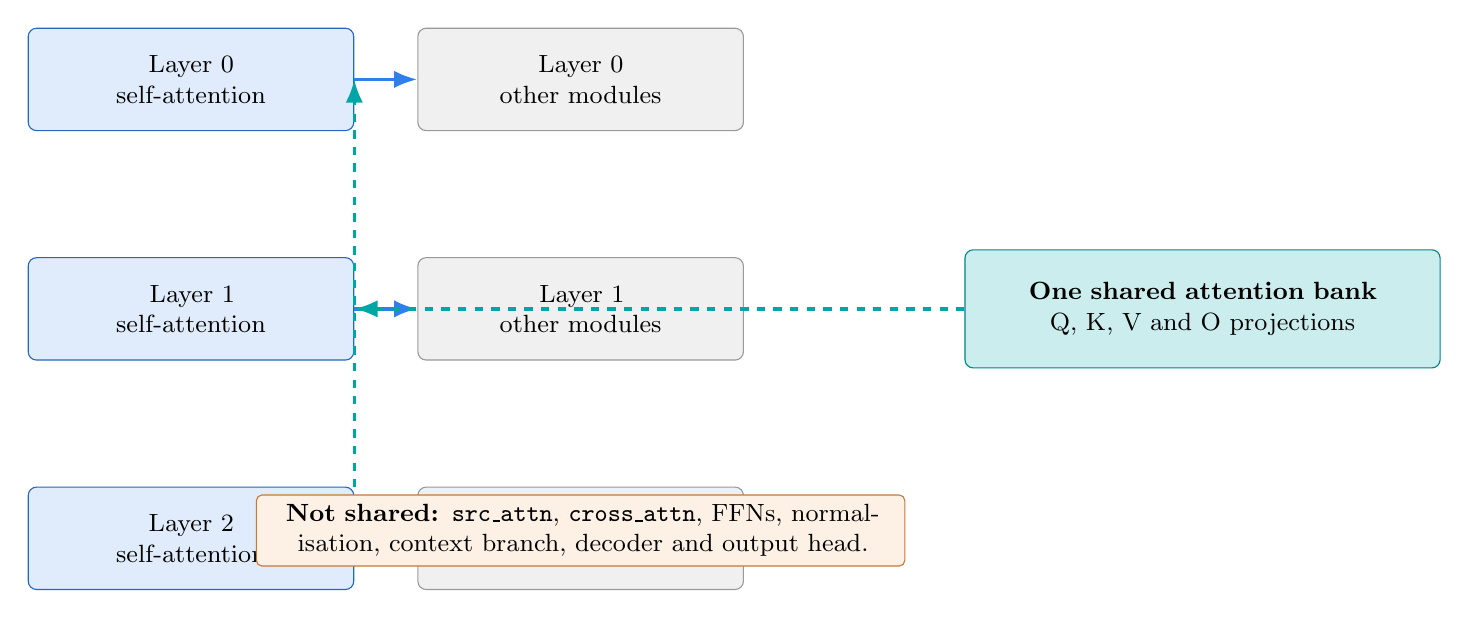
\begin{tikzpicture}[font=\small,
 attn/.style={draw=blue!80!black,fill=blue!15,rounded corners=3pt,minimum height=13mm,text width=39mm,align=center},
 other/.style={draw=gray!80,fill=gray!12,rounded corners=3pt,minimum height=13mm,text width=39mm,align=center},
 bank/.style={draw=teal!80!black,fill=teal!20,rounded corners=3pt,minimum height=15mm,text width=58mm,align=center},
 a/.style={-Latex,very thick,draw=blue},d/.style={-Latex,dashed,very thick,draw=teal}]
\node[attn] (s0) {Layer 0\\self-attention};\node[other,right=8mm of s0](r0){Layer 0\\other modules};
\node[attn,below=16mm of s0](s1){Layer 1\\self-attention};\node[other,right=8mm of s1](r1){Layer 1\\other modules};
\node[attn,below=16mm of s1](s2){Layer 2\\self-attention};\node[other,right=8mm of s2](r2){Layer 2\\other modules};
\draw[a](s0)--(r0);\draw[a](s1)--(r1);\draw[a](s2)--(r2);
\node[bank,right=28mm of r1] (bank) {\textbf{One shared attention bank}\\Q, K, V and O projections};
\draw[d](bank.west)-|(s0.east);\draw[d](bank.west)--(s1.east);\draw[d](bank.west)-|(s2.east);
\node[draw=orange!80!black,fill=orange!14,rounded corners=2pt,align=center,text width=80mm,below=17mm of r1] {\textbf{Not shared:} \texttt{src\_attn}, \texttt{cross\_attn}, FFNs, normalisation, context branch, decoder and output head.};
\end{tikzpicture}
}
\caption{C4 selective cross-layer sharing. Only encoder self-attention Q/K/V/O projections are tied across depth; remaining modules are independent.}
\label{fig:c4-sharing}
\end{figure*}

\begin{figure*}[t]
\centering
\resizebox{\textwidth}{!}{% Token append / decoder detail with a simple token visual.
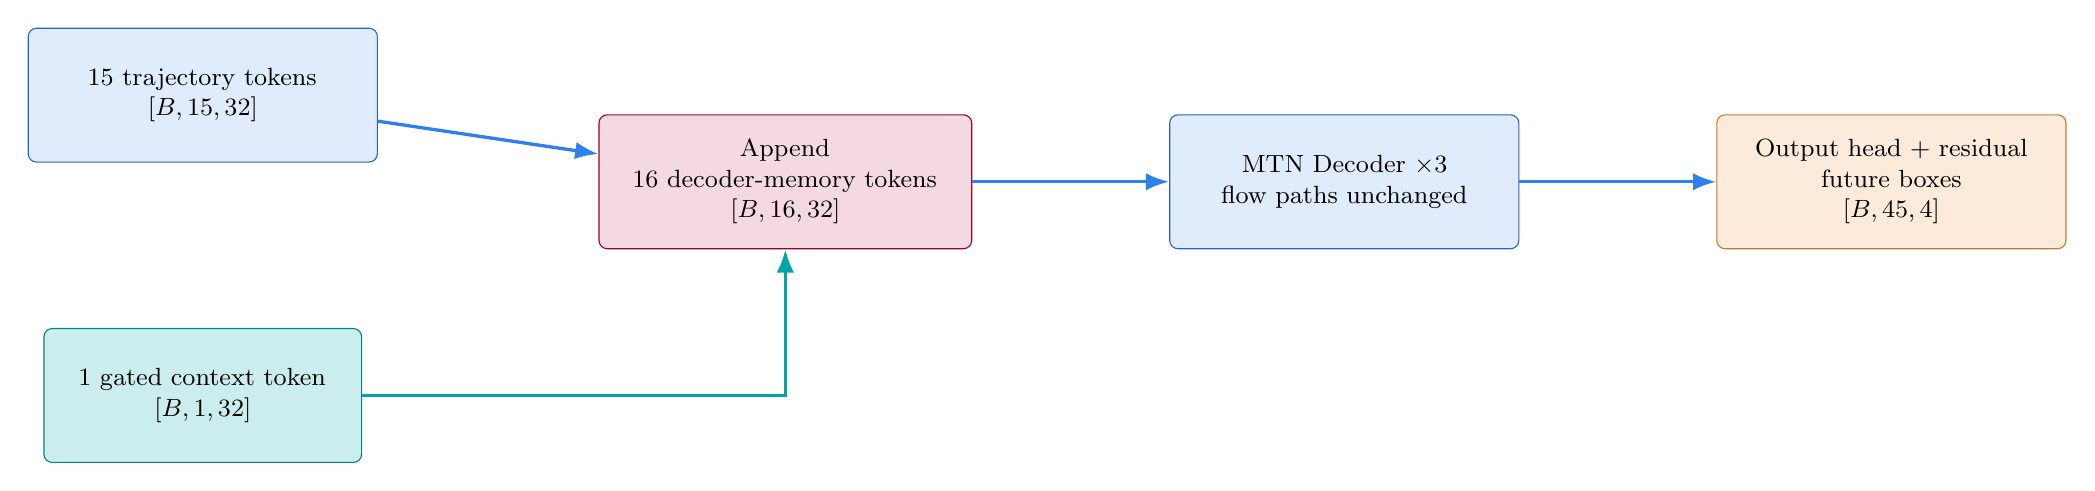
\begin{tikzpicture}[font=\small,
 mem/.style={draw=blue!80!black,fill=blue!15,rounded corners=3pt,minimum height=17mm,text width=42mm,align=center},
 tok/.style={draw=teal!80!black,fill=teal!20,rounded corners=3pt,minimum height=17mm,text width=38mm,align=center},
 aug/.style={draw=purple!80!black,fill=purple!15,rounded corners=3pt,minimum height=17mm,text width=45mm,align=center},
 outputbox/.style={draw=orange!80!black,fill=orange!20,rounded corners=3pt,minimum height=17mm,text width=42mm,align=center},
 a/.style={-Latex,very thick,draw=blue},ca/.style={-Latex,very thick,draw=teal}]
\node[mem](memory){15 trajectory tokens\\$[B,15,32]$};
\node[tok,below=21mm of memory](token){1 gated context token\\$[B,1,32]$};
\node[aug,right=28mm of memory,yshift=-11mm](append){Append\\16 decoder-memory tokens\\$[B,16,32]$};
\node[mem,right=25mm of append](decoder){MTN Decoder $\times3$\\flow paths unchanged};
\node[outputbox,right=25mm of decoder](output){Output head + residual\\future boxes\\$[B,45,4]$};
\draw[a](memory)--(append);\draw[ca](token.east)-|(append.south);\draw[a](append)--(decoder);\draw[a](decoder)--(output);
\end{tikzpicture}
}
\caption{Decoder-memory augmentation. The gated context becomes the sixteenth decoder-memory token without replacing the original 15 trajectory tokens.}
\label{fig:c4-memory}
\end{figure*}

\subsection{Novel contributions}
\begin{enumerate}[leftmargin=*,label=\textbf{C\arabic*.}]
\item \textbf{Context-token augmentation of MTN.} The method introduces six verified IDD-PeD context sources as a gated 32-dimensional decoder-memory token without replacing the trajectory pathway.
\item \textbf{Selective, technically scoped encoder sharing.} C4 ties only encoder self-attention Q/K/V/O across depth. This avoids incorrectly claiming that all encoder/decoder components are shared or that FLOPs decrease.
\item \textbf{Matched evidence-driven architecture selection.} B, C4, F, and F+C4 were evaluated under a common small CPU protocol, enabling a factual comparison of accuracy, variation across seeds, parameter count, and latency.
\end{enumerate}

\subsection{Separate Dynamic Multimodal Fusion candidate}
Dynamic Multimodal Fusion (F) was implemented and evaluated separately. It uses six 32-dimensional context tokens for cross-attention and a separate global context vector. The trajectory memory acts as query, while the six context tokens are keys and values. Identity, additive, and cross-attention candidates are computed, then a $64\rightarrow32\rightarrow3$ gate selects one operation per sample using hard Gumbel-Softmax in training and argmax/one-hot selection in evaluation. All three candidates are currently computed before selection; therefore F has no branch-skipping or resource-aware computational-saving claim. F is not included in the C4 proposed architecture in Figure~\ref{fig:c4-overview}.

\section{Experimental Results}
\label{sec:results}

\subsection{Protocol and reporting boundary}
The completed unified experiment used a fixed 32/8/24 train/validation/test trajectory split from locally available IDD-PeD data, CPU Farneback optical flow, Adam with learning rate 0.001, batch size 8, MSE loss, one training epoch, and three random seeds (20260928, 20260929, and 20260930). The test set comprises 24 trajectories from one held-out video. Reported values are mean $\pm$ sample standard deviation across the three seeds. This is a CPU-based proof-of-concept, not an official RAFT-based IDD-PeD benchmark reproduction.

\begin{figure*}[t]
\centering
\resizebox{\textwidth}{!}{% POC protocol figure; only uses completed experiment facts.
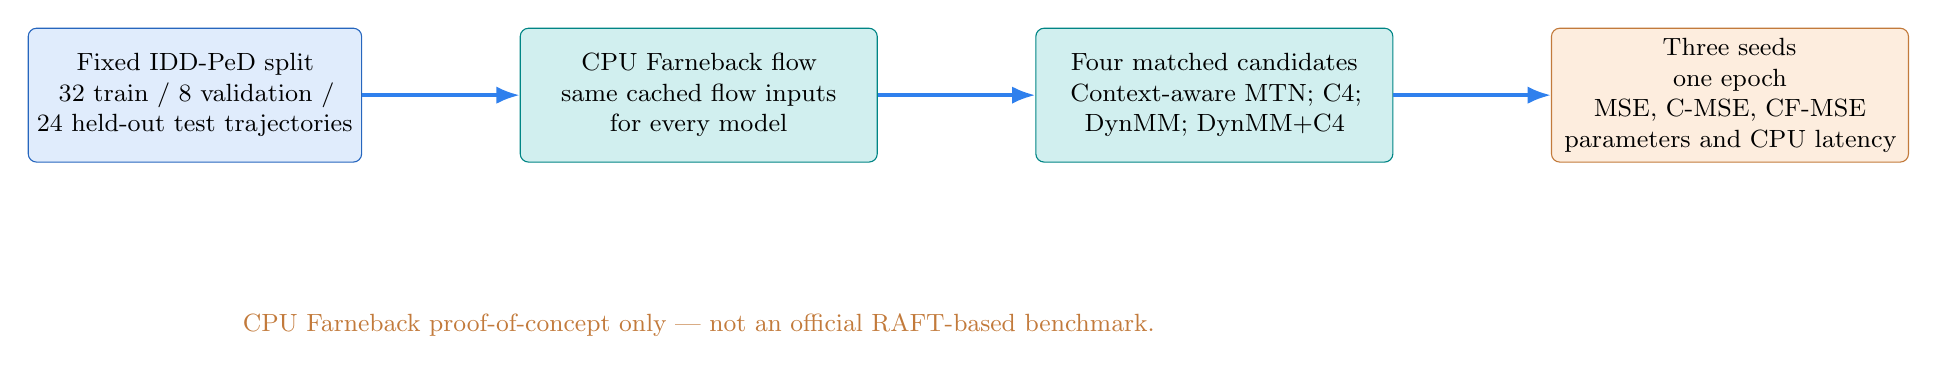
\begin{tikzpicture}[font=\small,
 d/.style={draw=blue!80!black,fill=blue!15,rounded corners=3pt,minimum height=17mm,text width=40mm,align=center},
 m/.style={draw=teal!80!black,fill=teal!18,rounded corners=3pt,minimum height=17mm,text width=43mm,align=center},
 r/.style={draw=orange!80!black,fill=orange!18,rounded corners=3pt,minimum height=17mm,text width=43mm,align=center},
 a/.style={-Latex,very thick,draw=blue}]
\node[d](split){Fixed IDD-PeD split\\32 train / 8 validation /\\24 held-out test trajectories};
\node[m,right=20mm of split](flow){CPU Farneback flow\\same cached flow inputs\\for every model};
\node[m,right=20mm of flow](models){Four matched candidates\\Context-aware MTN; C4;\\DynMM; DynMM+C4};
\node[r,right=20mm of models](eval){Three seeds\\one epoch\\MSE, C-MSE, CF-MSE\\parameters and CPU latency};
\draw[a](split)--(flow);\draw[a](flow)--(models);\draw[a](models)--(eval);
\node[font=\small,text=orange!80!black,below=18mm of flow] {CPU Farneback proof-of-concept only — not an official RAFT-based benchmark.};
\end{tikzpicture}
}
\caption{Matched CPU proof-of-concept protocol used for the completed unified experiment.}
\label{fig:protocol}
\end{figure*}

\begin{table*}[t]
\centering
\footnotesize
\caption{Unified matched \poc\ results. Lower MSE, C-MSE, CF-MSE, parameter count, and latency are better.}
\label{tab:unified}
\begin{tabular}{lrrrrr}
\toprule
Model & MSE & C-MSE & CF-MSE & Parameters & CPU latency (ms)\\
\midrule
B & $1137.11\pm20.16$ & $1107.40\pm19.63$ & $2971.36\pm103.13$ & 139,142 & $45.58\pm3.23$\\
C4 & $\mathbf{1080.16\pm93.33}$ & $\mathbf{1053.83\pm95.13}$ & $\mathbf{2887.51\pm237.14}$ & \textbf{130,694} & $47.38\pm2.48$\\
F & $1154.78\pm9.95$ & $1124.20\pm10.08$ & $3098.16\pm137.74$ & 154,007 & $50.68\pm2.48$\\
F+C4 & $1126.67\pm30.84$ & $1098.43\pm27.25$ & $3111.62\pm85.57$ & 145,559 & $52.07\pm4.74$\\
\bottomrule
\end{tabular}
\end{table*}

\subsection{Discussion of matched results}
C4 achieved the lowest mean MSE, C-MSE, and CF-MSE in this matched \poc. Relative to B, C4 changed MSE by $-5.01\%$, C-MSE by $-4.84\%$, and CF-MSE by $-2.82\%$, while reducing unique parameters by $6.07\%$. Its mean CPU latency was $3.93\%$ higher than B. The effect is not uniformly dominant per seed: C4 attained lower MSE than B in two of three seeds, while its MSE standard deviation was substantially larger ($93.33$ versus $20.16$). Thus, the evidence supports C4 as the current proposed \poc\ architecture, not a final universal selection.

F did not improve the measured prediction metrics over B: its relative changes were $+1.55\%$ MSE, $+1.52\%$ C-MSE, and $+4.27\%$ CF-MSE, accompanied by $+10.68\%$ parameters and $+11.18\%$ CPU latency. F+C4 reduced mean MSE by $0.92\%$ relative to B but increased CF-MSE by $4.72\%$, parameters by $4.61\%$, and latency by $14.23\%$. These results do not justify including F or F+C4 in the current proposed C4 architecture.

\subsection{Comparison with prior work on IDD-PeD}
Table~\ref{tab:prior} reports the published 1.5-second IDD-PeD trajectory-baseline results from the official paper \cite{iddped2025}. The published MTN, BiTraP, and SGNet results use the authors' approximately 70/30 train/test split, RAFT optical flow for MTN, GPU hardware, and the full test set. In contrast, our completed comparison uses CPU Farneback flow, one held-out video, 24 trajectories, one epoch, and three seeds. Therefore, the table is a \emph{dataset-context comparison}, not a direct numerical ranking of our method against the published baselines.

\begin{table*}[t]
\centering
\scriptsize
\caption{Published IDD-PeD baselines at 1.5 seconds and the current CPU POC. Lower is better. The final row is not directly comparable with the published rows because the protocol differs.}
\label{tab:prior}
\setlength{\tabcolsep}{3pt}
\begin{tabular}{p{0.27\textwidth}p{0.24\textwidth}rrr}
\toprule
Source / protocol & Method & MSE & C-MSE & CF-MSE\\
\midrule
Official IDD-PeD paper; full test split; RAFT/GPU & PIETraj & 2181 & 1979 & 8960\\
Official IDD-PeD paper; full test split; RAFT/GPU & MTN & 1652 & 1489 & 6668\\
Official IDD-PeD paper; full test split; published setup & BiTraP & 338 & 200 & 638\\
Official IDD-PeD paper; full test split; published setup & SGNet & 310 & 190 & 531\\
\midrule
Current work; CPU Farneback POC, 24 trajectories, one epoch & Context-Aware MTN with Encoder Self-Attention Sharing & $1080.16\pm93.33$ & $1053.83\pm95.13$ & $2887.51\pm237.14$\\
\bottomrule
\end{tabular}
\end{table*}

The current POC has lower numerical error than the published deterministic MTN baseline, but this must not be interpreted as a benchmark improvement because flow representation, train/test scale, training budget, and hardware differ. The appropriate current conclusion is limited: within the matched local POC, encoder self-attention sharing improved mean error metrics relative to the local Context-Aware MTN reference. A direct comparison against published work requires reproducing the official split and RAFT pipeline.

\section{Ablation Study}
\label{sec:ablation}

The ablation study is organised around completed experiments already documented in the project tracker. Results from different POC protocols are not merged into a single ranking; the unified 12-run ablation is the primary matched comparison.

\begin{figure*}[t]
\centering
\resizebox{\textwidth}{!}{% Ablation design, distinguished from results and future work.
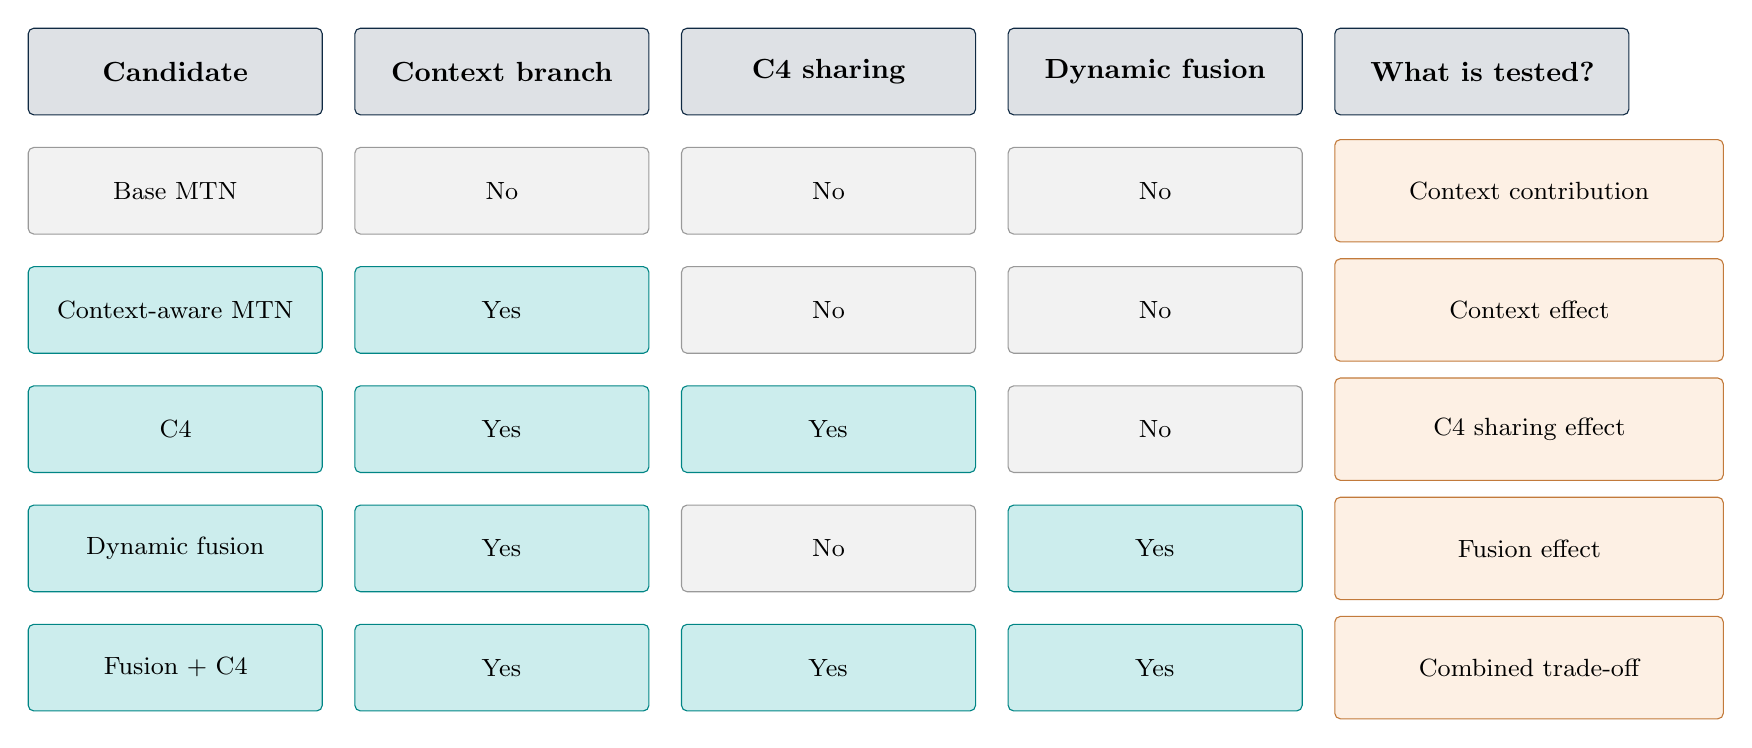
\begin{tikzpicture}[font=\small,
 h/.style={draw=navy,fill=navy!14,rounded corners=2pt,minimum height=11mm,text width=35mm,align=center,font=\bfseries},
 yes/.style={draw=teal!80!black,fill=teal!20,rounded corners=2pt,minimum height=11mm,text width=35mm,align=center},
 no/.style={draw=gray!80,fill=gray!10,rounded corners=2pt,minimum height=11mm,text width=35mm,align=center},
 note/.style={draw=orange!80!black,fill=orange!15,rounded corners=2pt,minimum height=13mm,text width=47mm,align=center}]
\node[h](c0){Candidate};\node[h,right=4mm of c0](c1){Context branch};\node[h,right=4mm of c1](c2){C4 sharing};\node[h,right=4mm of c2](c3){Dynamic fusion};\node[h,right=4mm of c3](c4){What is tested?};
\node[no,below=4mm of c0](r1){Base MTN};\node[no,right=4mm of r1](r11){No};\node[no,right=4mm of r11](r12){No};\node[no,right=4mm of r12](r13){No};\node[note,right=4mm of r13](r14){Context contribution};
\node[yes,below=4mm of r1](r2){Context-aware MTN};\node[yes,right=4mm of r2](r21){Yes};\node[no,right=4mm of r21](r22){No};\node[no,right=4mm of r22](r23){No};\node[note,right=4mm of r23](r24){Context effect};
\node[yes,below=4mm of r2](r3){C4};\node[yes,right=4mm of r3](r31){Yes};\node[yes,right=4mm of r31](r32){Yes};\node[no,right=4mm of r32](r33){No};\node[note,right=4mm of r33](r34){C4 sharing effect};
\node[yes,below=4mm of r3](r4){Dynamic fusion};\node[yes,right=4mm of r4](r41){Yes};\node[no,right=4mm of r41](r42){No};\node[yes,right=4mm of r42](r43){Yes};\node[note,right=4mm of r43](r44){Fusion effect};
\node[yes,below=4mm of r4](r5){Fusion + C4};\node[yes,right=4mm of r5](r51){Yes};\node[yes,right=4mm of r51](r52){Yes};\node[yes,right=4mm of r52](r53){Yes};\node[note,right=4mm of r53](r54){Combined trade-off};
\end{tikzpicture}
}
\caption{Ablation design: each candidate isolates the contribution of native context, C4 sharing, dynamic fusion, or their combination.}
\label{fig:ablation-design}
\end{figure*}

\subsection{Context contribution: original MTN versus B}
An early paired \poc\ compared original MTN (A) with context-aware MTN (B) on 10 held-out trajectories from GP6 video 3, using one seed, 12 epochs, and CPU Farneback flow. A obtained MSE 1242.98, C-MSE 1225.17, CF-MSE 4093.85, and latency 69.24 ms. B obtained MSE 1113.21, C-MSE 1094.57, CF-MSE 3646.51, and latency 61.41 ms. This preliminary result motivated retaining the context branch. It is not directly comparable with the later unified one-epoch, three-seed experiment.

\subsection{Full sharing versus targeted sharing}
Full encoder-and-decoder sharing reduced parameters from 139,142 to 53,894 ($61.3\%$) but increased MSE from 1113.21 to 1339.31 and increased latency from 47.20 to 50.13 ms in its recorded POC. It was therefore rejected. This supports testing selective sharing rather than tying entire layers.

\begin{table*}[t]
\centering
\scriptsize
\caption{Targeted weight-sharing POC. C3 was not run because the current decoder has no active decoder self-attention. C5 was not run because genuine head sharing requires a new projection parameterisation.}
\label{tab:targeted}
\begin{tabular}{llrrrr}
\toprule
Variant & Sharing scope & Parameters & MSE & C-MSE & CF-MSE / latency (ms)\\
\midrule
B & None & 139,142 & 972.51 & 949.45 & 2802.67 / 47.79\\
C1 & Decoder src\_attn Q/K/V/O & 130,694 & 1081.44 & 1049.76 & 3369.58 / 53.68\\
C2a & Decoder src\_attn Q/K/V & 132,806 & 1188.92 & 1169.76 & 3940.10 / 56.30\\
C2b & Decoder src\_attn K/V & 134,918 & 1152.49 & 1133.15 & 3807.02 / 47.99\\
C4 & Encoder self\_attn Q/K/V/O & 130,694 & 819.99 & 798.82 & 2441.16 / 49.56\\
\bottomrule
\end{tabular}
\end{table*}

\subsection{Unified architecture ablation}
The primary ablation is Table~\ref{tab:unified}, which compares B, C4, F, and F+C4 under the same split, seed set, optimiser, loss, epoch budget, and CPU flow cache. It separately tests: (i) C4 encoder self-attention sharing, (ii) F dynamic multimodal fusion, and (iii) their combination. This design demonstrates component contributions without changing the evaluation protocol between compared variants.

\subsection{Interpretation and remaining ablations}
The evidence indicates that selective C4 sharing is more promising than full sharing, decoder-targeted sharing, or the currently implemented F fusion. However, the observed C4 variance and latency increase require broader validation. The next ablation, if approved, should retain the same architecture and evaluate across additional held-out videos and a reproduced RAFT/GPU setting. It should measure the same MSE, C-MSE, CF-MSE, parameter count, latency, and seed-level variation. No additional result is claimed in this draft.

\section{Limitations and Next Steps}
The draft has four key limitations. First, CPU Farneback flow differs from the authors' RAFT pipeline. Second, the unified \poc\ uses one held-out video and 24 trajectories. Third, models were trained for one epoch, so the comparison is not a convergence study. Fourth, C4 reduces unique parameters but does not reduce FLOPs because all encoder attention operations execute; F computes all fusion candidates before selecting one.

The immediate next steps are supervisor review of the C4 and F diagrams, integration of the selected C4 figure and text into the manuscript, and broader validation only if requested. The published values currently shown in Table~\ref{tab:prior} should remain labelled as a dataset-context comparison; they should be used for direct numerical ranking only after the official split, flow pipeline, training budget, and evaluation hardware are reproduced.

\bibliographystyle{plain}
\bibliography{references}
\end{document}
